In this section, we compare $\latentranker$ to several bandit algorithms in three experiments. The first two experiments are on synthetic dataset where all modeling assumptions hold. The third experiment is on a real-life dataset where we evaluate $\latentranker$ when our modeling assumptions fail. In all our experiments user come uniform randomly over all time $[n]$. All results are averaged over $10$ independent random runs.

\subsection{Evaluated Algorithms}
\textbf{Independent User Model Algorithms:} In this approach, each user has a separate version of base-bandit algorithm running independent of each other. As base-bandit algorithms we choose two variants of the ranked bandit algorithm ($\RBA$) of \citet{radlinski2008learning}. The two variants of $\RBA$ uses two types of column learning algorithms, $\ucb$ \citep{auer2002finite} and $\expthree$ \citep{auer2002nonstochastic}, abbreviated as $\RBAUCB$ and $\RBAEXP$ respectively. $\expthree$ is a randomized algorithm suited for the adversarial setting while $\ucb$ is the standard algorithm used in the stochastic feedback setting. For $\RBAUCB$, we choose the confidence interval at time $t$ as $c_{i, j}(t) = \sqrt{\frac{ 2\log t}{N_{i, j}(t)}}$ for user $i$ and item $j$. Here, $N_{i, j}(t)$ denotes the number of times the $j$-th item has been observed by the $i$-th user base-bandit algorithm till timestep $t$. Note, that running independent vanilla $\ucb$ and $\expthree$ for every user is not feasible. This is because the vanilla versions are guaranteed to find a single best item for each user at rank $1$, while $\RBAUCB$ and $\RBAEXP$ will find a diverse list of $d$ best items for each user.

%it suggest previously unselected items by sampling uniform randomly at each time $t$. \todob{Why? This does not seem fair. We need to change baselines. I have an idea.}


\textbf{Matrix Completion Algorithms:} In the matrix completion approach, the algorithms try to reconstruct the user-item preference matrix $M$ from its noisy realization. We implement the widely used non-negative matrix factorization method to reconstruct partially observed noisy matrices. We term the corresponding algorithm as NMF Bandit ($\NMFBan$). The objective function of $\NMFBan$ is:-
\begin{align*}
\text{minimize} \norm{\hat{M} - \hat{U}\hat{V}^\intercal}_{F}^{2} \text{with respect to $\hat{U}, \hat{V}$}\\
\text{ subject to constraints } \hat{U}, \hat{V} \geq 0
\end{align*}

where, $\hat{M}$ is the observed noisy matrix of size $K \times L$ which has a low rank $d$, $\hat{U} \in [0,1]^{K \times d}$ and $\hat{V} \in [0,1]^{L \times d}$ are estimated non negative matrices which  generates $\hat{M}$ such that $\hat{M} \approx \hat{U}\hat{V}^{\intercal}$. This objective function is minimized by alternating minimization of $\hat{U}$ and $\hat{V}$ till the loss is very low. $\NMFBan$ knows the rank of the matrix $\hat{M}$. This algorithm is explore-exploit in implementation whereby it first explores for $cd(K + L)$ rounds by choosing items for incoming users uniform randomly, where $c$ is an exploration parameter which can be tuned depending on the noise in the system. We set $c=10$ in all experiments. Then it reconstructs $\hat{M}$ using the objective function mentioned above. Then over the reconstructed matrix it behaves greedily and suggest $d$ best item for the $i_t$-th user at every timestep $t$. 

%Note, that NMF-Ban needs to sufficiently explore the noisy realizations of the matrix $\hat{M}$ before it reconstructs. For this reason, we set the $\epsilon$ very low such that $\epsilon = 10^{-5}$.


%After exploring for some timesteps (depending on the exploration parameter) it calls the reconstruction function above with \hat{M}, to get an estimate of the U and V. Then it reconstructs \hat{M} from that U and V.
%
%3) Then, at every timestep t, when an user i comes, it suggests d items in descending order of preference from \hat{M}(i,:). Do you have any suggestion to improve it
%
%%This is done till the loss is very low (1e-4) or till 200 iteration. The matrices are initialized randomly.
%
%We term the corresponding algorithm as NMF Bandit (NMF-Ban). This algorithm is $\epsilon$-greedy in implementation whereby it reconstructs $M$ with $\epsilon$ probability and with $1-\epsilon$ probability it behaves greedily over the reconstructed matrix and suggest $d$ best item for the $i_t$-th user at every timestep $t$. Note, that NMF-Ban needs to sufficiently explore the noisy realizations of the matrix $M$ before it reconstructs. For this reason, we set the $\epsilon$ very low such that $\epsilon = 10^{-5}$.

%\todob{I thought that we do explore-exploit. In any case, say what $\epsilon$ / exploration horizon is.}

\textbf{Personalized Ranking Algorithms:} In this approach, we evaluate our proposed algorithm latent ranking bandit ($\latentranker$) by using three different types of column learning algorithms, $\expthree$, thompson sampling  \citep{thompson1933likelihood}, \citep{thompson1935theory}, \citep{agrawal2012analysis} and \ucb. We term them as $\LRAEXP$, $\LRATS$ and $\LRAUCB$ respectively. Note, that thompson sampling is a Bayesian algorithm that performs better than $\ucb$ in stochastic setting due to its inherent prior assumptions on the distribution of the feedback. The row ranking components for all of these algorithms is the weighted majority algorithm ($\WMA$) from \citet{littlestone1994weighted} which is suited for the full information setting. Note that we only show theoretical guarantees for $\LRAEXP$. We initialize the $k$-th column EXP3 with the column exploration parameter $\gamma_k = \sqrt{\frac{L \log L}{n}}$ as stated in \citet{auer2002nonstochastic}. Similarly, for $\LRAUCB$ we use  a confidence interval of $c_{k, j}(t) = \sqrt{\frac{2\log t}{N_{k,j}(t)}}$  for the $k$-th column MAB and $j$-th item. Here, $N_{k, j}(t)$ denotes the number of times the $j$-th item has been observed by the $k$-th column $\ucb$ algorithm till timestep $t$.

%Note, that for all the versions of UCB1 used in several types of algorithms we use an aggressive confidence interval to enhance the performance of these  algorithms. This is contrary to the conservative confidence interval used to prove theoretical guarantees in \citet{auer2002finite}.

%\todob{$\gamma_k$ was never defined before. Why do you need to introduce it now?}

%\todob{The name of this setting is super confusing. If you say contextual, people expect feature vectors. We have no feature vectors. Say independent model for each user. That is clear and says precisely what we do.}
%
%\todosb{Changed this to Independent User Model Algorithms}

%\textbf{Matrix Completion Algorithms:} In the matrix completion approach, the algorithms try to reconstruct the user-item preference matrix $M$ from its noisy realization. We implement the widely used method to reconstruct partially observed noisy matrices, the non-negative matrix factorization. We term the corresponding algorithm as NMF Bandit (NMF-Ban). This algorithm is $\epsilon$-greedy in implementation whereby it reconstructs $M$ with $\epsilon$ probability and with $1-\epsilon$ probability it behaves greedily over the reconstructed matrix and suggest $d$ best item for the $i_t$-th user at every timestep $t$. 

%LinBan uses ridge regression to reconstruct $M$ from its estimated $d$-best columns while NMF-Ban uses matrix factorization to estimate the $U$ and $V$ matrix and reconstruct $M$ from its noisy realization. \todob{It is absolutely not clear what LinBan does.}

%\textbf{Personalized Ranking Algorithms:} In this approach, we evaluate our proposed algorithm Latent Ranking Bandit (LRA) by using two different types of Column MABs, EXP3 and UCB1. We term them as LREXP3 and LRUCB1 respectively. The row ranking components for both of these algorithms is still Weighted Majority Algorithm (WMA). Note that we only show theoretical guarantees for LREXP3. For LREXP3 we set the column exploration parameter $\gamma_k = \sqrt{\frac{L \log L}{n}}, \forall \text{ MAB}_k(n), k = 1,\dots, d$ and for LRUCB1 we use  a confidence interval of $c_{k, j}(t) = \sqrt{\frac{1.5 \log t}{N_{k,j}(t)}}$ for the $k$-th column MAB and $j$-th item.

%\todob{What? We do not do this anymore, no? Why is it here? It makes no sense to use a bandit algorithm since we are in the full-observation setting. No UCB1 please. Exp3 should be weighted majority.}

\subsection{Synthetic Experiment $1$}
This experiment is conducted to test the performance of $\latentranker$ over small number of users and items. This simulated testbed consist of $500$ users, $50$ items, and rank$(M) = 2$. The vectors spanning $U$ and $V$, generating the user-item preference matrix $M$, are shown Figure \ref{fig:1}. The users are evenly distributed into a $50:50$ split such that $50\%$ of users prefer item $1$ and $50\%$ users prefer item  $2$. The item hott-topics are $V(1,:) = (0,1)$ and $V(2,:) = (1, 0)$ while remaining $70\%$ of items has feature $V(j',:) = (0.45, 0.55)$ and the rest have $V(j,:) = (0.55, 0.45)$. We create the user feature matrix $U$ similarly having a $50:50$ split such that $U(1,:) = (0,1)$, $U(2,:) = (0.2,0.8)$ and the remaining $70\%$ users having $U(i,:) = (0,0.8)$ and $30\%$ users having $U(i',:) = (0.7,0)$. At every timestep $t$ the resulting matrix $M_t =UD_tV^{\intercal}$ is generated where $D_t$ is a randomly-generated diagonal matrix. So, $M_t$ is  such that algorithms that quickly find the easily identifiable hott-topics perform very well. From Figure \ref{fig:2} we can clearly see that $\LRAEXP$, $\LRATS$ and $\LRAUCB$ outperforms all the other algorithms. Their regret curve flattens, indicating that they have learned the best items for each user. Independent user model algorithms $\RBAUCB$ and $\RBAEXP$  perform poorly as the number of items per user is too large and the independent algorithms are not sharing information between them. $\NMFBan$ performs better than the independent user model algorithms but is outperformed by $\LRAEXP$, $\LRATS$ and $\LRAUCB$.

%well in this small testbed but its performance degrades for larger datasets.

%Although CTS performs well in this small testbed, its performance eventually degrades for larger environments. 

%\todob{Again, we never defined $j^\ast_1$ and $j^\ast_2$ before. Why do you think that an unexplained notation is better than explaining this in plain English?}


\begin{figure}[!th]
\centering
\begin{tabular}{cc}
\setlength{\tabcolsep}{0.1pt}
\subfigure[0.25\textwidth][Expt-$1$: $500$ Users, $50$ items, Rank $2$, User and Item vectors]
    %with $r_{i_{{i}\neq {*}}}=0.07$ and $r^{*}=0.1$
    {
    		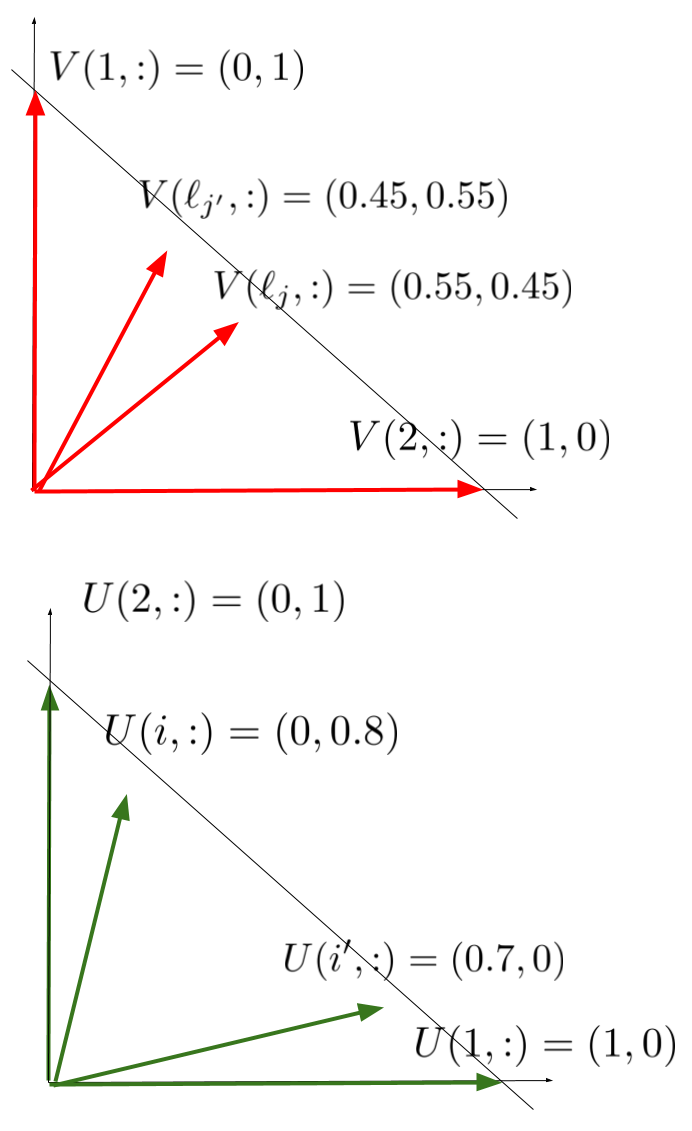
\includegraphics[scale=0.11]{img/rank2_vec.png}
  		\label{fig:1}
    }
    &
    \subfigure[0.25\textwidth][Expt-$1$: Cumulative regret of different algorithms]
    %with $r_{i_{{i}\neq {*}}}=0.07$ and $r^{*}=0.1$
    {
    		\pgfplotsset{
		tick label style={font=\Large},
		label style={font=\Large},
		legend style={font=\Large},
		ylabel style={yshift=5pt},
		%legend style={legendshift=32pt},
		}
        \begin{tikzpicture}[scale=0.4]
      	\begin{axis}[
		xlabel={timestep},
		ylabel={Cumulative Regret},
		grid=major,
        %clip mode=individual,grid,grid style={gray!30},
        clip=true,
        %clip mode=individual,grid,grid style={gray!30},
        cycle list name=exotic,
  		legend style={at={(0.5,1.4)},anchor=north, legend columns=3} ]
      	% UCB
		%\addplot table{results/NewExpt1/Expt11/comp_subsampled_CTS0RR1S.txt};
		\addplot table{results/NewExpt3/Expt1/comp_subsampled_RBAEXP30RR1S.txt};
		\addplot table{results/NewExpt3/Expt1/comp_subsampled_LRTS0RR1S.txt};
		\addplot table{results/NewExpt3/Expt1/comp_subsampled_LRUCB0RR1S.txt};
		\addplot table{results/NewExpt3/Expt1/comp_subsampled_LREXP30RR1S.txt};
		\addplot table{results/NewExpt3/Expt1/comp_subsampled_NMFEE0RR1S.txt};
		%\addplot table{results/NewExpt1/Expt1/comp_subsampled_LinBan0RR1S.txt};
		%\addplot table{results/NewExpt1/Expt11/comp_subsampled_CUCB10RR1S.txt};
		\addplot table{results/NewExpt3/Expt1/comp_subsampled_RBAUCB10RR1S.txt};
		\legend{RBA-EXP3, LRA-TS, LRA-UCB1, LRA-EXP3, NMF-Ban, RBA-UCB1} 
      	\end{axis}
      	\end{tikzpicture}
  		\label{fig:2}
    }
    \\
    \subfigure[0.25\textwidth][Expt-$2$: $1500$ Users, $100$ items, Rank $3$, User and Item vectors]
    %with $r_{i_{{i}\neq {*}}}=0.07$ and $r^{*}=0.1$
    {
    		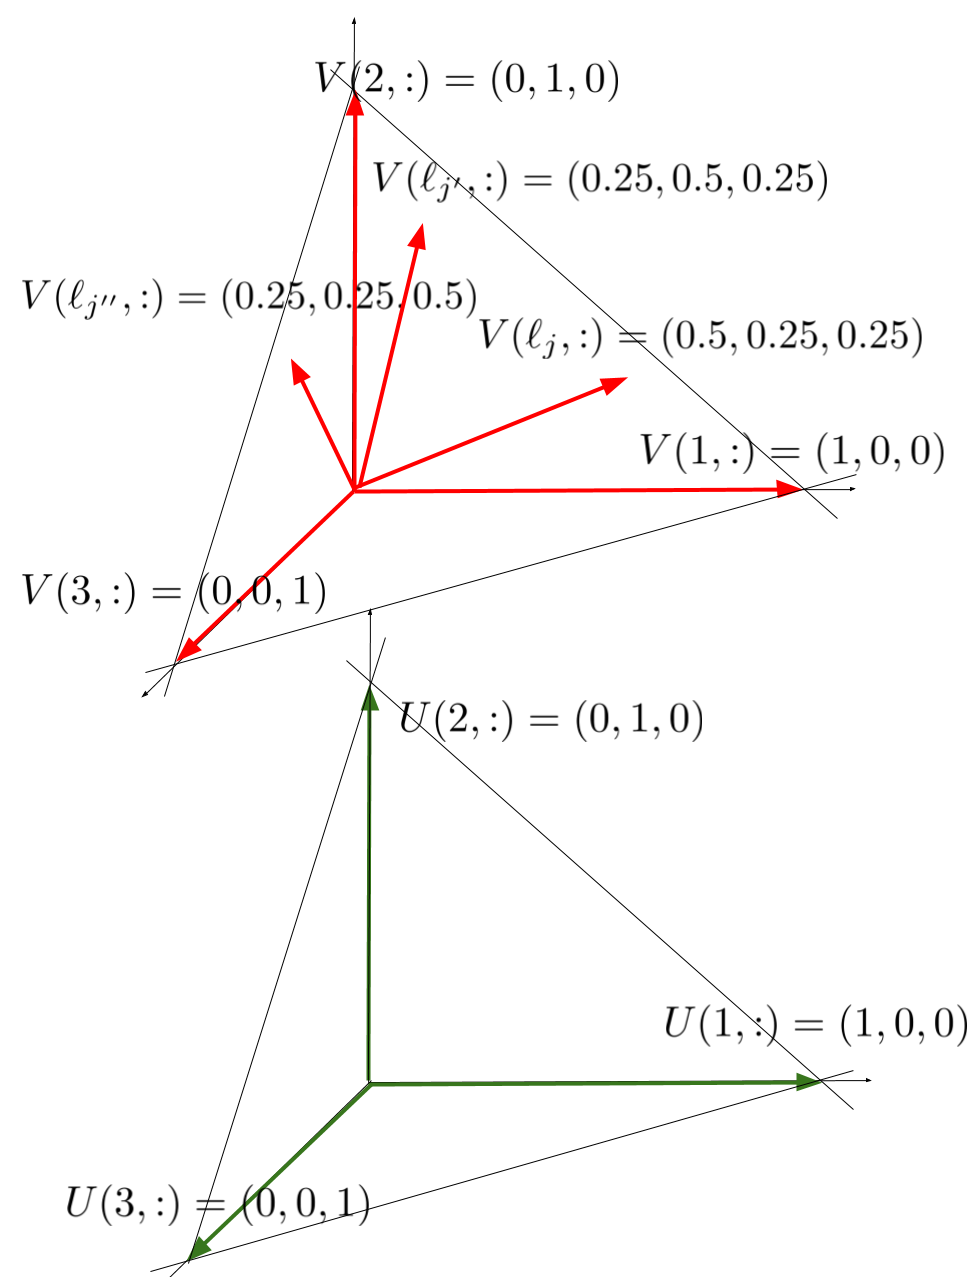
\includegraphics[scale=0.11]{img/rank3_vec.png}
  		\label{fig:3}
    }
    &
    \subfigure[0.25\textwidth][Expt-$2$: Cumulative regret of different algorithms]
    %with $r_{i_{{i}\neq {*}}}=0.07$ and $r^{*}=0.1$
    {
    		\pgfplotsset{
		tick label style={font=\Large},
		label style={font=\Large},
		legend style={font=\Large},
		ylabel style={yshift=5pt},
		%legend style={legendshift=32pt},
		}
        \begin{tikzpicture}[scale=0.4]
      	\begin{axis}[
		xlabel={timestep},
		ylabel={Cumulative Regret},
		grid=major,
        %clip mode=individual,grid,grid style={gray!30},
        clip=true,
        %clip mode=individual,grid,grid style={gray!30},
        cycle list name=exotic,
  		legend style={at={(0.5,1.4)},anchor=north, legend columns=3} ]
      	% UCB
		%\addplot table{results/NewExpt1/Expt11/comp_subsampled_CTS0RR1S.txt};
		\addplot table{results/NewExpt3/Expt2/comp_subsampled_RBAEXP30RR1S.txt};
		\addplot table{results/NewExpt3/Expt2/comp_subsampled_LRTS0RR1S.txt};
		\addplot table{results/NewExpt3/Expt2/comp_subsampled_LRUCB0RR1S.txt};
		\addplot table{results/NewExpt3/Expt2/comp_subsampled_LREXP30RR1S.txt};
		\addplot table{results/NewExpt3/Expt2/comp_subsampled_NMFEE0RR1S.txt};
		%\addplot table{results/NewExpt1/Expt1/comp_subsampled_LinBan0RR1S.txt};
		%\addplot table{results/NewExpt1/Expt11/comp_subsampled_CUCB10RR1S.txt};
		\addplot table{results/NewExpt3/Expt2/comp_subsampled_RBAUCB10RR1S.txt};
		\legend{RBA-EXP3, LRA-TS, LRA-UCB1, LRA-EXP3, NMF-Ban, RBA-UCB1} 
      	\end{axis}
      	\end{tikzpicture}
  		\label{fig:4}
    }
    \end{tabular}
    \caption{A comparison of the cumulative regret incurred by the various bandit algorithms. }
    \label{fig:karmed1}
    \vspace*{-1em}
\end{figure}

%\todob{Why two pictures? Why do you subindex some $V$ with $\ell_j$?}]
%\todob{Why two pictures? Why do you subindex some $V$ with $\ell_j$?}]

\subsection{Synthetic Experiment $2$}
We conduct the second experiment on a larger simulated database of $1500$ users, $100$ items and rank$(M)=3$. The vectors spanning $U$ and $V$, generating the user-item preference matrix $M$ is shown Figure \ref{fig:3}. The users are divided into an unequal distribution of $60:30:10$ split such that $60\%$ of the users prefer item item $1$, $30\%$ prefer item $2$ and $10\%$ prefer item $3$. Hence, in this testbed it is difficult to learn item $3$ as it is observed for less number of users. Here, hott-topics are $V(1,:) = (1,0,0)$, $V(2,:) = (0,1, 0)$ and $V(3,:) = (0,0,1)$. The remaining $60\%$ of items have feature  $V(j,:) = (0.5, 0.25,0.25)$, $30\%$ have $V(j',:) = (0.25, 0.5, 0.25)$ and rest have $V(j^{''},:) = (0.25, 0.25, 0.5)$. We create the user feature matrix $U$ similarly having a $60:30:10$ split and the vectors spanning $U$ are only of the type that spans the simplex, i.e $U(i,:)=(1,0,0)$, $U(i',:)=(1,0,0)$ and $U(i^{''},:)=(1,0,0)$. Again, at every timestep $t$ the resulting matrix $M_t =UD_tV^{\intercal}$ is generated where $D_t$ is a randomly-generated diagonal matrix. So, $M_t$ is  such that algorithms that quickly find the easily identifiable hott-topics perform very well. From Figure \ref{fig:4} we can see that $\LRAEXP$, $\LRATS$ and $\LRAUCB$ again outperform all the other algorithms. Their regret curve flattens much before all the other algorithms indicating that they have learned the best items for each user. The matrix completion algorithm $\NMFBan$ again fails to get a reasonable approximation of $M$ and performs poorly. Also, we see that both the independent user model algorithms $\RBAUCB$ and $\RBAEXP$ perform poorly as the number of users and the number of items per user is too large and the independent base-bandits ($\RBA$) are not sharing information between themselves. In both the synthetic datasets, we see that stochastic column learning algorithm ($\ucb$) is outperforming adversarial column learning algorithm ($\expthree$) as the user preference over the best item is not changing over time. This has also been observed by \citet{radlinski2008learning}.

%which stems from the fact that all the user, 

%%%%%%% Rank 4 grouping %%%%
%[548, 99], [266, 93], [262, 96], [250, 28], [142, 59], [135, 79], [96, 88], [55, 78], [52, 9], [26, 52], [24, 76], [23, 67], [23, 68], [23, 95], [20, 97], [19, 66], [10, 40], [9, 7], [9, 85], [3, 1], [3, 17], [2, 61]

\subsection{Real World Experiment $3$}
We conduct the third experiment to test the performance of LRA when our modelling assumptions are violated. We use the Jester dataset \citep{goldberg2001eigentaste} which consist of over 4.1 million continuous ratings of 100 jokes from 73,421 users collected over 5 years. In this dataset there are many users who rated all jokes and we work with these users. Hence the user-item preference matrix is fully observed and we will not have to complete it using matrix completion techniques. Hence, this approach is very real world. We sample randomly $2000$ users (who have rated all jokes) from this dataset and use singular value decomposition (SVD) to obtain a rank $4$ approximation of this user-joke rating matrix $M$. In the resultant matrix $M$, most of the users belong to the four classes preferring jokes 99, 93, 96 and 28, while a very small percentage of users prefer some other jokes. Note, that this condition results from the fact that this real-life dataset does not have the hott-topics structure. The rank $4$ approximation of $M$ of  is shown in Figure \ref{fig:5}, where we can clearly see the red stripes spanning the matrix indicating the low-rank structure of $M$. Furthermore, in this experiment we assume that the noise is independent Bernoulli over the entries of $M$ and hence this experiment deviates from our modeling assumptions. From \ref{fig:6} again we see that $\LRAEXP$, $\LRATS$ and $\LRAUCB$ outperform other algorithms. Although the cumulative regret of $\NMFBan$ is less than our proposed approaches, note that it does not converge and find the $d$ best items.

%The regret curve of LRA-UCB1 does not flatten out which we attribute to the fact that LRA-UCB1 uses too large a confidence interval. The contextual and matrix completion algorithms perform significantly worse in this large testbed.

%\todob{The rank should be chosen using cross-validation. How do you know that rank $2$ is good?}

%[[1104, 99], [896, 93],[0,0][0,0]}

\begin{figure}[!th]
\centering
\begin{tabular}{cc}
\setlength{\tabcolsep}{0.1pt}
\subfigure[0.25\textwidth][Expt-$3$: $2000$ Users, $100$ items, Rank $4$ approximation of Jester Dataset]
    %with $r_{i_{{i}\neq {*}}}=0.07$ and $r^{*}=0.1$
    {
    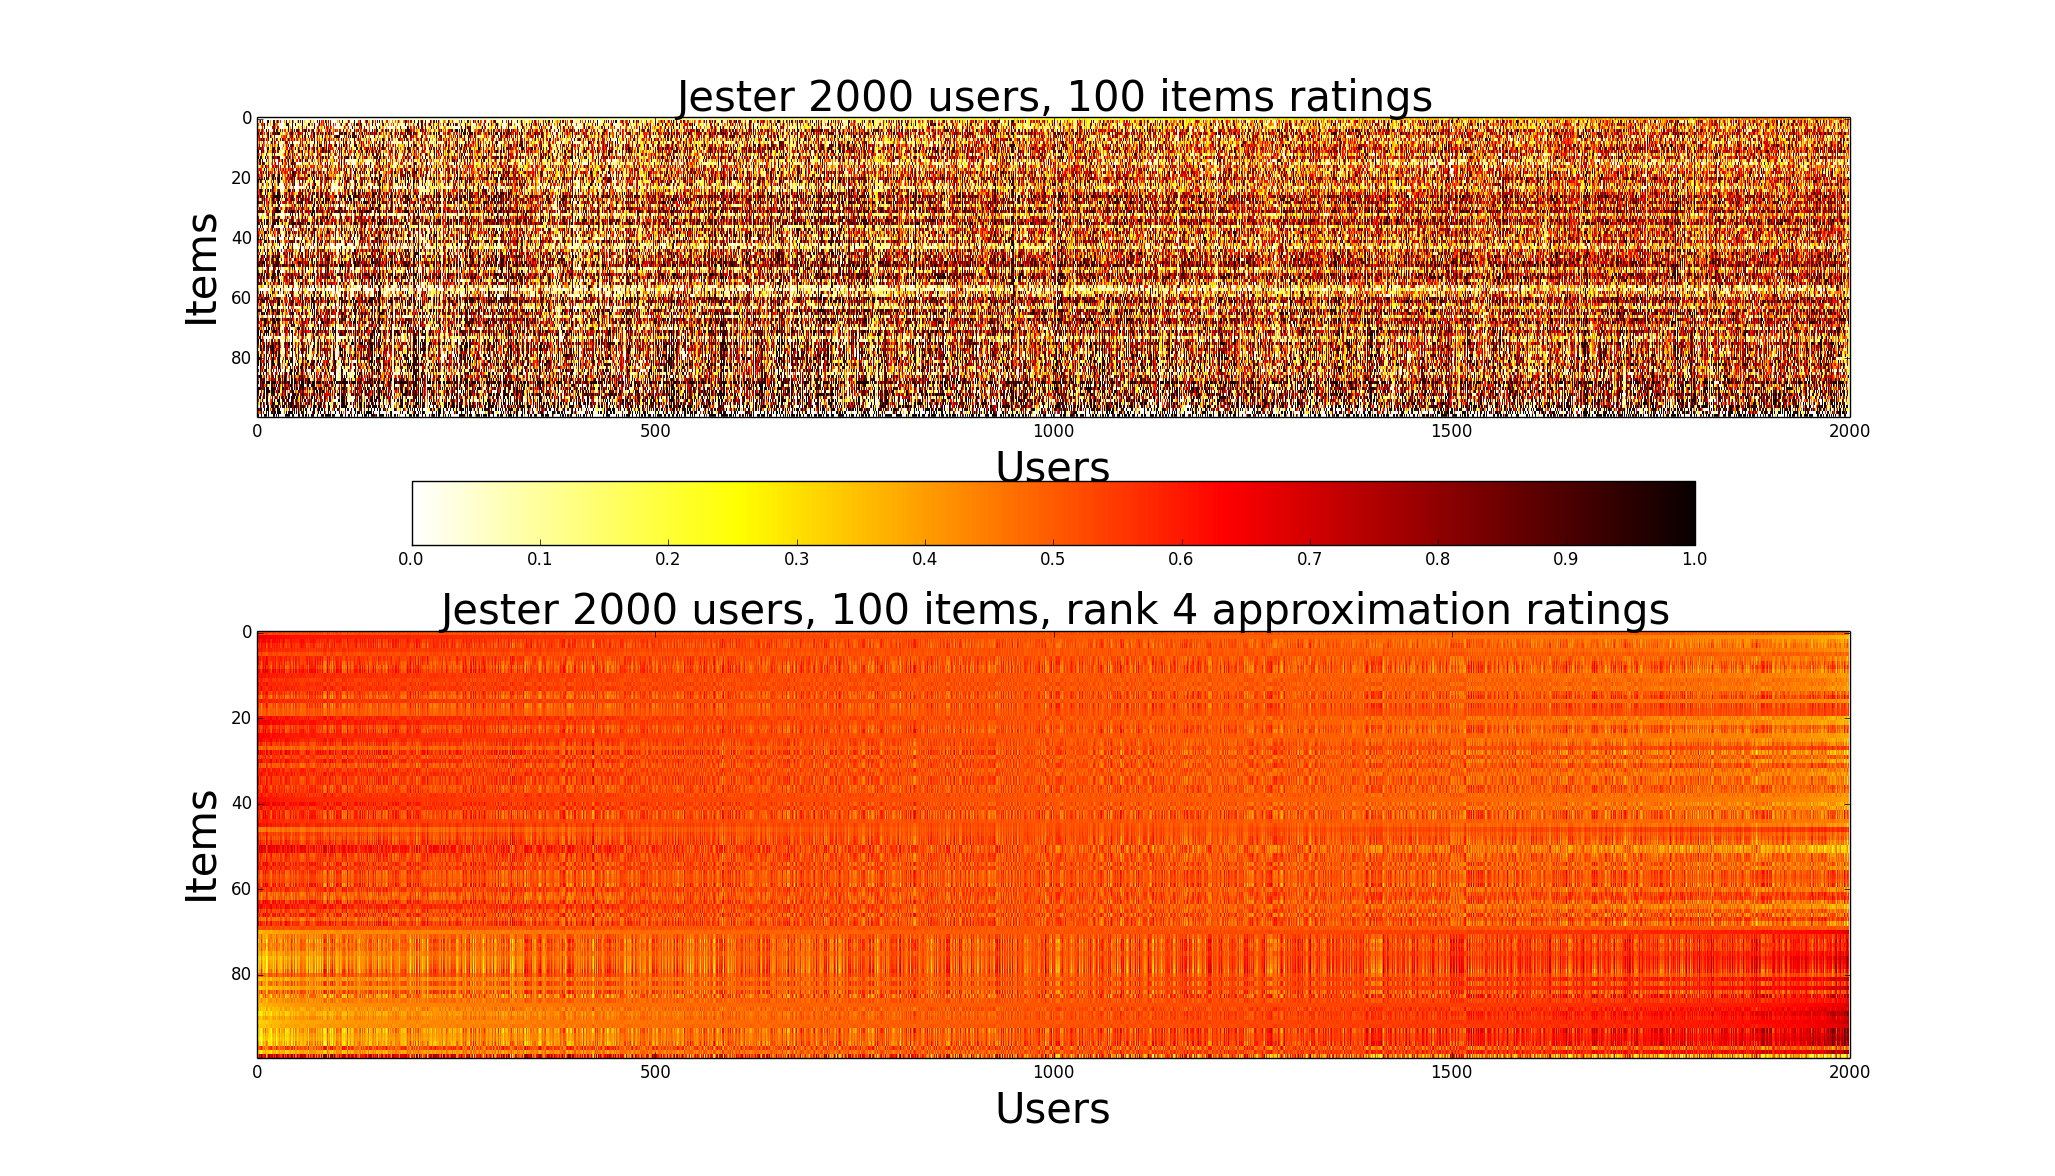
\includegraphics[scale=0.08]{img/jester_rank4.png}
    	\label{fig:5}
    }
    &
\subfigure[0.25\textwidth][Expt-$3$: Cumulative regret of different algorithms]
    %with $r_{i_{{i}\neq {*}}}=0.07$ and $r^{*}=0.1$
    {
    		\pgfplotsset{
		tick label style={font=\Large},
		label style={font=\Large},
		legend style={font=\Large},
		ylabel style={yshift=5pt},
		%legend style={legendshift=32pt},
		}
        \begin{tikzpicture}[scale=0.4]
      	\begin{axis}[
		xlabel={timestep},
		ylabel={Cumulative Regret},
		grid=major,
        %clip mode=individual,grid,grid style={gray!30},
        clip=true,
        cycle list name=exotic,
        %clip mode=individual,grid,grid style={gray!30},
  		legend style={at={(0.5,1.4)},anchor=north, legend columns=3} ]
      	% UCB
		%\addplot table{results/NewExpt1/Expt11/comp_subsampled_CTS0RR1S.txt};
		\addplot table{results/NewExpt3/Expt3/comp_subsampled_RBAEXP30RR1S.txt};
		\addplot table{results/NewExpt3/Expt3/comp_subsampled_LRTS0RR1S.txt};
		\addplot table{results/NewExpt3/Expt3/comp_subsampled_LRUCB0RR1S.txt};
		\addplot table{results/NewExpt3/Expt3/comp_subsampled_LREXP30RR1S.txt};
		\addplot table{results/NewExpt3/Expt3/comp_subsampled_NMFEE0RR1S.txt};
		%\addplot table{results/NewExpt1/Expt1/comp_subsampled_LinBan0RR1S.txt};
		%\addplot table{results/NewExpt1/Expt11/comp_subsampled_CUCB10RR1S.txt};
		\addplot table{results/NewExpt3/Expt3/comp_subsampled_RBAUCB10RR1S.txt};
		\legend{RBA-EXP3, LRA-TS, LRA-UCB1, LRA-EXP3, NMF-Ban, RBA-UCB1} 
      	\end{axis}
      	\end{tikzpicture}
  		\label{fig:6}
    }
 \end{tabular}
    \caption{A comparison of the cumulative regret in Jester Dataset }
    \label{fig:karmed}
    \vspace*{-1em}
\end{figure}